\documentclass[aspectratio=169,11pt]{beamer}
% Shared preamble for the CogLean decks.
% Build the slides alone, or with speaker notes (see the Makefile):
%   pdflatex deck.tex                                   -> slides
%   pdflatex -jobname=deck-notes "\def\withnotes{}\input{deck.tex}"  -> slides + notes
\usetheme{default}
\usecolortheme{seahorse}
\setbeamertemplate{navigation symbols}{}
\setbeamertemplate{footline}[frame number]
\setbeamerfont{note page}{size=\small}
\ifdefined\withnotes
  \setbeameroption{show notes}
\fi
\usepackage[T1]{fontenc}
\usepackage{lmodern}
\usepackage{booktabs}
\usepackage{amsmath,amssymb}
\usepackage{tikz}
\usetikzlibrary{positioning,arrows.meta,shapes.misc}
\tikzset{
  box/.style={draw, rounded corners, align=center, minimum height=8mm, inner sep=4pt, fill=blue!6},
  arr/.style={-{Stealth[length=2mm]}, thick}
}
\newcommand{\code}[1]{\texttt{#1}}
\newcommand{\has}{\textbf{has}}
\newcommand{\lacks}{\textcolor{red!70!black}{lacks}}
\newcommand{\never}{\textcolor{red!70!black}{\textbf{never}}}
\newcommand{\canhold}{can hold}


\title{A blind simulation of a formalized theory}
\subtitle{Checking that the definitions say what the theory says}
\author{Jeff Shrager}
\date{October 2026}

\begin{document}

\begin{frame}
  \titlepage
\end{frame}
\note{
This is a methods talk about a question every formal model faces: does the formalization say what the theory says? The procedure I'll describe doesn't need Lean or any theorem prover. All the materials, the specification, the preregistration, the delivered simulator, the harness and the results, are in the repository.
}

\begin{frame}{The question}
  A Lean proof shows that a prediction follows from the \emph{definitions}.
  \bigskip

  It does not show that the definitions say what the \emph{theory} says.
  \bigskip
  \begin{itemize}
    \item The theory: postulates in prose (EPAM's discrimination nets, distributions of associations, multi-digit addition).
    \item The formalization: one reading of that prose, made precise.
    \item Every theorem inherits whatever the reading got wrong.
  \end{itemize}
  \bigskip
  How can the link between the prose and the formal definitions be checked?
\end{frame}
\note{
A Lean proof shows that a prediction follows from the definitions. It doesn't show that the definitions say what the theory says. The theory lives in prose; the formalization is one reading of that prose, made precise; and every theorem inherits whatever that reading got wrong. This is the first objection a skeptical audience raises, and it's fair: machine-checked proofs move the risk from the derivation to the definitions. Simulation papers have the same problem in another form, since the published description and the code can differ.
}

\begin{frame}{The idea: two independent readings}
  \centering
  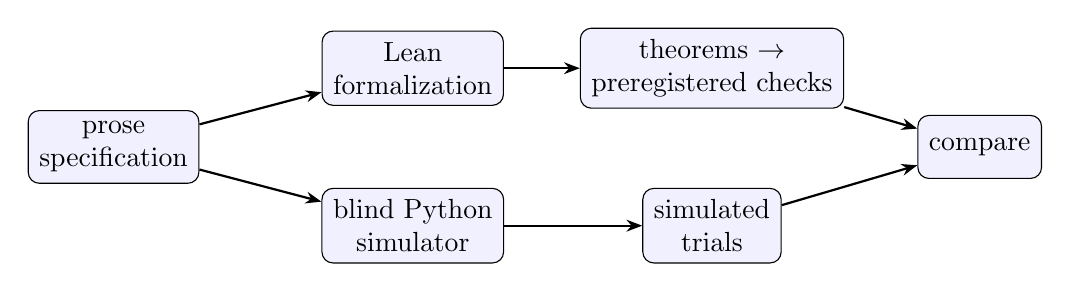
\begin{tikzpicture}
    \node[box] (spec) at (0,0) {prose\\specification};
    \node[box] (lean) at (3.8,1) {Lean\\formalization};
    \node[box] (py) at (3.8,-1) {blind Python\\simulator};
    \node[box] (pred) at (7.6,1) {theorems $\to$\\preregistered checks};
    \node[box] (logs) at (7.6,-1) {simulated\\trials};
    \node[box] (cmp) at (11,0) {compare};
    \draw[arr] (spec) -- (lean); \draw[arr] (spec) -- (py);
    \draw[arr] (lean) -- (pred); \draw[arr] (py) -- (logs);
    \draw[arr] (pred) -- (cmp); \draw[arr] (logs) -- (cmp);
  \end{tikzpicture}
  \bigskip
  \raggedright

  N-version programming (Avi\v{z}ienis 1985), applied to a theory. A disagreement means one of three things: the prose is ambiguous, the formalization drifted, or the simulator has a bug.
\end{frame}
\note{
We borrowed an idea from fault-tolerant software, called N-version programming: build two independent implementations of one specification, and look at where they disagree. Here, one reading of the prose is the Lean formalization, whose theorems give predictions. The other is a Python simulator written without seeing any of the Lean. If they disagree, then either the prose is ambiguous, the formalization drifted, or the simulator has a bug, and in every case we learn something.
}

\begin{frame}{The procedure}
  \begin{enumerate}
    \item \textbf{A prose specification} (\code{SPEC.md}): the model in plain words, with no Lean names, theorems, or predictions. Points the prose leaves open are listed as \emph{open choices}.
    \item \textbf{A preregistration} (\code{PREREG.md}): each theorem's observable statistic and how it is judged. Committed \emph{before} the simulator existed; the implementer never saw it.
    \item \textbf{A blind implementer}: a fresh AI agent, given only the specification, in an empty directory. Its tool calls were audited: it read only files it had written.
    \item \textbf{Lean's exact distributions} for four shared instances.
    \item \textbf{A harness} (\code{compare.py}): random instances, the preregistered checks, and a report.
  \end{enumerate}
  \medskip
  \small Commits, 26 October 2026: specification and preregistration 19:16; simulator, unmodified, 19:21; harness and results 19:31.
\end{frame}
\note{
Concretely: we wrote a prose specification with no Lean in it, and we listed explicitly the points the prose leaves open. We preregistered the predictions, committing them before the simulator existed. Then a fresh AI agent, given only the prose, wrote the simulator in an empty directory, and we audited its tool use to check that it read nothing else. Lean exported exact probability distributions for some shared cases, and a harness compared everything. The commit timestamps show the order: the specification and preregistration first, the simulator five minutes later, the results ten minutes after that.
}

\begin{frame}{Open choices, declared in advance}
  The specification names the points the prose leaves open; the implementer must choose, document the choice, and expose it as a parameter.
  \medskip
  \begin{itemize}
    \item \textbf{O1.} When strengthening after a whole-problem answer, is ``correct'' judged against the problem's true sum, or the sum of the problem whose associations were used?
    \item \textbf{O2.} What associations does a newly discriminated problem start with?
    \item \textbf{O3.} Does an answer computed by the columns change the whole-problem associations?
    \item \textbf{O4.} Anything else found underdetermined.
  \end{itemize}
\end{frame}
\note{
A key step was to declare, in advance, the points the prose leaves open, and to require the implementer to choose, document and parameterize each one. For instance: when strengthening after a whole-problem answer, is correctness judged against the problem's true sum, or the sum of the problem whose associations were used? What associations does a newly discriminated problem start with? Does an answer computed by the columns change the whole-problem associations? Declaring these separates the theory not saying from the implementer getting it wrong, and one of them turned out to matter a great deal.
}

\begin{frame}{How each check is judged}
  \begin{itemize}
    \item \textbf{Exact relations}: zero violations allowed, over every trial whose hypothesis holds. For example, an error is the confused neighbour's answer.
    \item \textbf{Probabilities}: pass if $|\hat p - p| < 4\sqrt{p(1-p)/N}$. For example, column use $= (1-R)^n$.
    \item \textbf{No-change and monotone relations}: for example, learning other problems leaves a practiced problem's trial unchanged.
    \item \textbf{Non-vacuity}: each check reports how many trials met its hypothesis. A check whose hypothesis never held is reported as \emph{vacuous}, not as passed.
  \end{itemize}
  \medskip
  Instances: 4 Lean-exact; 30 random with learning off; 20 random with learning on, across the open choices.
\end{frame}
\note{
Each check was judged by a rule fixed in advance. Exact relations allow no violations at all, over every trial whose hypothesis holds. Probabilities pass if the observed frequency is within four standard errors of Lean's value. No-change relations, such as learning other problems leaving a practiced one untouched, are checked exactly. And there's a non-vacuity rule: every check reports how many trials met its hypothesis, and one whose hypothesis never held is reported as vacuous, not as passed. That rule is easy to forget, and it turned out to be essential.
}

\begin{frame}{Results: no failures}
  \small
  \begin{center}
  \resizebox{\linewidth}{!}{%
  \begin{tabular}{lllrr}
    \toprule
    Check & Lean theorem & kind & tests & failures\\
    \midrule
    Lean exact & \code{\#eval MD.trial} & prob & 243 & 0\\
    P1 & \code{columns\_prob} & prob & 394 & 0\\
    P2 & \code{whole\_depends\_only\_on\_route} & prob & 8543 & 0\\
    P3 & \code{confusion\_gives\_neighbours\_answer} & exact & 200 & 0\\
    P4 & \code{confident\_errors} & exact+prob & 222 & 0\\
    P7 & \code{learning\_preserves\_trial} & exact & 74692 & 0\\
    P9 & \code{columns\_place\_value} & exact & 248800 & 0\\
    P11 & \code{discrimination\_removes\_confusion} & exact & 91090 & 0\\
    P6a, P6b, P14, P17, P18 & & & 0 & \emph{vacuous}\\
    \bottomrule
  \end{tabular}}
  \end{center}
  \medskip
  \normalsize
  The prose and the formalization agree on recognition, EPAM learning, retrieval, both backups, and carrying.
\end{frame}
\note{
The result: no failures. 243 outcome frequencies matched Lean's exact values, and every applicable prediction passed, some of them over tens of thousands of trials. So the prose and the formalization agree on recognition, learning, retrieval, both backups and carrying. But look at the bottom row: five predictions were vacuous.
}

\begin{frame}{Finding 1: five predictions were never tested}
  \begin{itemize}
    \item Predictions 6a, 6b, 14, 17 and 18 need the net's path to test \emph{every} feature of a digit or a column: 4 bits, 9 thresholds, or 100 fact features.
    \item EPAM grows one test per confusion, so paths are short. In no learned net did the hypothesis ever hold.
    \item The theorems are true. But they say almost nothing about the nets EPAM actually learns.
  \end{itemize}
  \bigskip
  \textit{Lesson.} A theorem can be correct and nearly irrelevant to the models the theory produces. Restate it in terms of what learned nets do test: for example, ``the tested bits of a digit restrict it to a set''.
\end{frame}
\note{
That is the most interesting finding. Those five predictions needed the net to test every feature of a digit. But EPAM grows only one test per confusion, so in no learned net did that ever happen. The theorems are true, and yet they say almost nothing about the nets EPAM actually produces. That's a general lesson for proving things about cognitive models: the hypotheses that make a proof go through can quietly exclude the cases you care about. Without a rule that reports vacuous checks as vacuous, these would have looked like five passes.
}

\begin{frame}{Finding 2: a gap in the formalization}
  \begin{itemize}
    \item In Lean, sampling divides by total strength. With total strength 0, a trial has \emph{no} outcome at all: probability mass 0.
    \item The theorems avoid this by assuming total strength $\neq 0$.
    \item The simulator read it as ``retrieval exhausted, go to the columns''. That is the natural reading of the model.
    \item It matters: a newly discriminated problem with no associations (the most natural choice of O2) is exactly this case, and it lies outside every theorem.
  \end{itemize}
  \bigskip
  A gap in the formalization, not a simulator bug.
\end{frame}
\note{
The second finding is a gap in the formalization. In Lean, sampling divides by the total strength, so with a total of zero a trial has no outcome at all. The theorems avoid this by assuming the total isn't zero. The simulator read it as retrieval exhausted, go to the columns, which is the natural reading of the model. And it matters, because a newly discriminated problem with no associations, the most natural answer to one of the open choices, is exactly this case, and it lies outside every theorem. That's a gap in the formalization, not a bug in the simulator.
}

\begin{frame}{Finding 3: a prediction depends on an open choice}
  The predicted learning sequence: a confident error, then column work, then fluent correct retrieval.
  \medskip
  \small
  \begin{center}
  \resizebox{\linewidth}{!}{%
  \begin{tabular}{lrrrrr}
    \toprule
    O2: new problem starts with & discriminated & canonical & settles on correct & mixed & trapped on error\\
    \midrule
    no associations & 48 & 40 & 7 & 1 & 0\\
    only the correct answer & 61 & 28 & 33 & 0 & 0\\
    a copy of the neighbour's & 44 & 0 & 2 & 35 & 7\\
    \bottomrule
  \end{tabular}}
  \end{center}
  \medskip
  \normalsize
  \begin{itemize}
    \item With no associations, the predicted sequence appears (40 of 48).
    \item Starting with the correct answer, the column phase is often skipped.
    \item Copying the neighbour's associations perpetuates the error.
  \end{itemize}
\end{frame}
\note{
Another finding concerns learning. The model predicts a sequence: a confident error, then column work after feedback, then fluent, correct retrieval. But the model doesn't say what associations a newly discriminated problem starts with; that was one of the open choices we declared. And the sequence depends on it. Starting with no associations, the predicted sequence appears in 40 of 48 cases. Starting with only the correct answer, the column phase is often skipped. Copying the neighbour's associations perpetuates the error. So a substantive question about the theory has become sharp.
}

\begin{frame}{Finding 4: ambiguities resolved the same way, blind}
  The implementer met ambiguities the specification did not flag, and resolved them as the Lean formalization had:
  \begin{itemize}
    \item single-digit associations belong to \emph{ordered} pairs ($3+5$ and $5+3$ separately);
    \item whole-problem strengthening applies to the associations that were actually retrieved from.
  \end{itemize}
  \bigskip
  Agreement found independently is evidence that these are the natural readings, and it should have been in the specification.
\end{frame}
\note{
The fourth finding is reassuring. The implementer met two ambiguities that the specification didn't flag: whether single-digit associations belong to ordered pairs, so that 3 plus 5 and 5 plus 3 are separate, and whether strengthening applies to the associations that were actually retrieved from. It resolved both exactly as the Lean formalization does. Agreement reached independently is some evidence that these are the natural readings, though they should have been in the specification.
}

\begin{frame}{Limits}
  \begin{itemize}
    \item \textbf{Blindness is procedural.} It rests on instructions and an audit of tool calls, not on anything that prevents reading.
    \item \textbf{Not fully independent.} The implementer was a model of the same family as the one that wrote the specification and the formalization, so shared misreadings are possible. A human implementer, or community code, would be stronger.
    \item \textbf{One model, one round.} It checked the EPAM + DOA multi-digit model, before memory became a plug-in and before the ACT-R version existed.
    \item \textbf{Simulation covers instances.} It can expose a mismatch; it cannot certify the definitions in general.
  \end{itemize}
\end{frame}
\note{
The limits, stated plainly. Blindness here is procedural: it rests on instructions and an audit of the agent's tool calls, not on anything that physically prevents reading. The implementer was a model of the same family as the one that wrote the specification and the formalization, so shared misreadings are possible; a human implementer, or community code, would be stronger. It covered one model, in one round, before memory became a plug-in. And simulation covers instances: it can expose a mismatch, but it can't certify the definitions in general.
}

\begin{frame}{Next}
  \begin{itemize}
    \item \textbf{A second round for ACT-R's memory}: a prose specification of the activation family, a blind implementation, and preregistered checks from the matrix's ACT-R cells.
    \item \textbf{Community code as the second version}: compare the Lean ACT-R memory with PyACTUp, CMU's implementation. Blended retrieval should match exactly; noisy retrieval within tolerance.
    \item \textbf{A human implementer} for at least one round.
    \item \textbf{Standard practice}: every formalized theory in the library gets a prose specification and a blind check.
  \end{itemize}
  \bigskip
  \small The recipe (spec, open choices, preregistration, blind implementer, non-vacuity) needs no theorem prover. Any modelling group can use it.
\end{frame}
\note{
Next, a second round for ACT-R's memory: a prose specification of the activation family, a blind implementation, and preregistered checks from the matrix. Then community code as the second version: compare our ACT-R memory with PyACTUp, CMU's implementation, where blended retrieval should match exactly and noisy retrieval within tolerance. We'd like a human implementer for at least one round, and to make this standard practice for every theory in the library. And the recipe, a specification with declared open choices, a preregistration, a blind implementer and a non-vacuity rule, needs no theorem prover, so any modelling group can use it.
}

\end{document}
